\documentclass[12pt]{article}


\usepackage{amssymb}
\usepackage{amsmath}
\usepackage{fullpage}
\usepackage{epsfig}
\usepackage{epstopdf}
\everymath{\displaystyle}

\newif\ifans

\ansfalse

\begin{document}

\begin{center}
\underline{\LARGE{Chapter 4.2 (Part 2) \& 4.3 Practice Problems}}
\end{center}

\noindent EXPECTED SKILLS:

\begin{itemize}

\item Be able to use the extrema along with the end behavior (i.e. “dominant term”) of polynomials to sketch the graph of polynomial
functions.

\item Know how to determine if the graph of a function has a cusp or vertical tangent line at a point (i.e. the function is not differentiable at that point).  And, be able to use this information, along with extrema, intercepts, and asymptotes, to sketch the graph of a function.

\end{itemize}

\noindent PRACTICE PROBLEMS:

\medskip

\noindent {\bf For problems 1-12, sketch the given functions.  Label  the coordinates of all critical points, inflection points, $x$-intercepts, $y$-intercepts, and holes.  Also label all horizontal asymptotes and vertical asymptotes}

\begin{enumerate}

\item $f(x)=x^2(x^2-4)$

\fbox{\parbox{1\linewidth}{\begin{center}
$f(x)=x^4-4x^2$; $f^{\prime}(x)=4x^3-8x$; $f^{\prime \prime}(x)=12x^2-8$\\
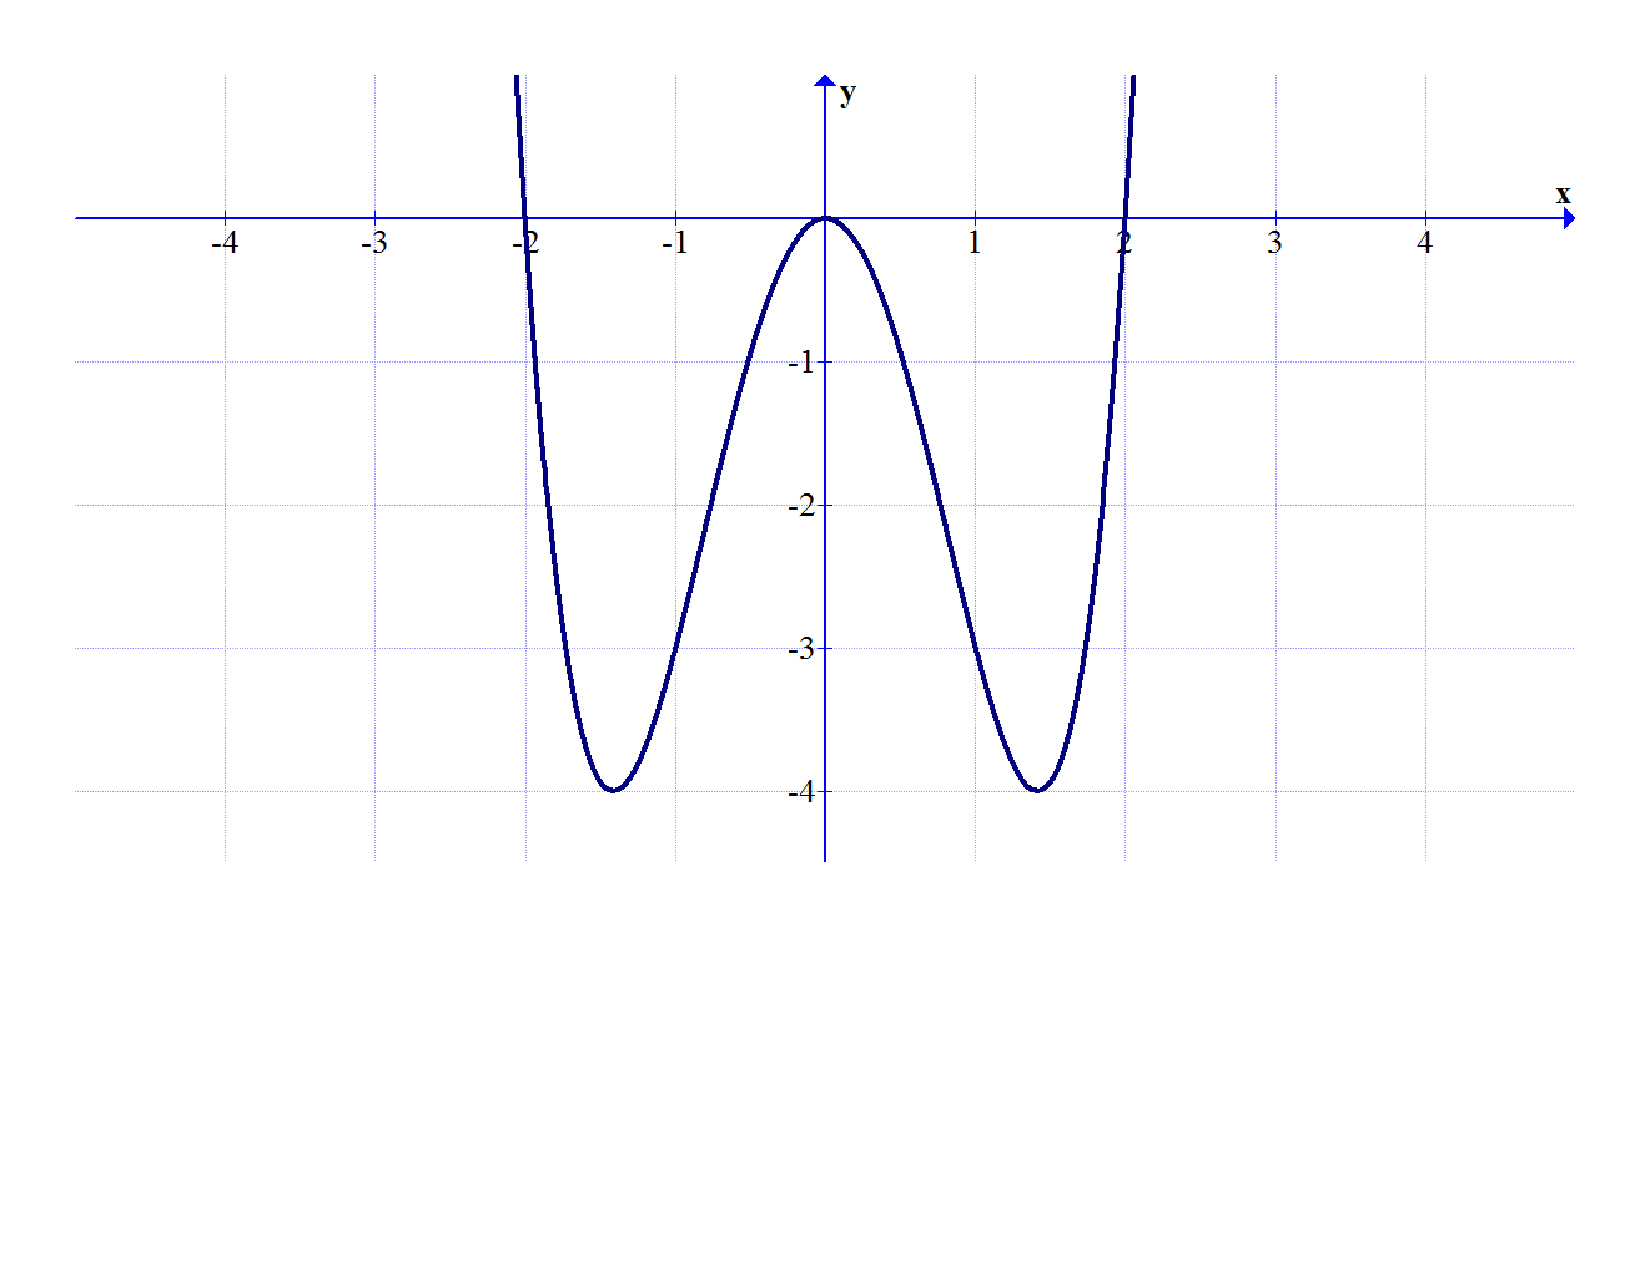
\includegraphics[scale=0.25]{1.pdf}
\end{center}
}}

\item $f(x)=x^3+7x^2+8x-16$\\
(HINT: $f(1)=0$)

\fbox{\parbox{1\linewidth}{\begin{center}
$f(x)=x^3+7x^2+8x-16$; $f^{\prime}(x)=3x^2+14x+8$; $f^{\prime \prime}(x)=6x+14$\\
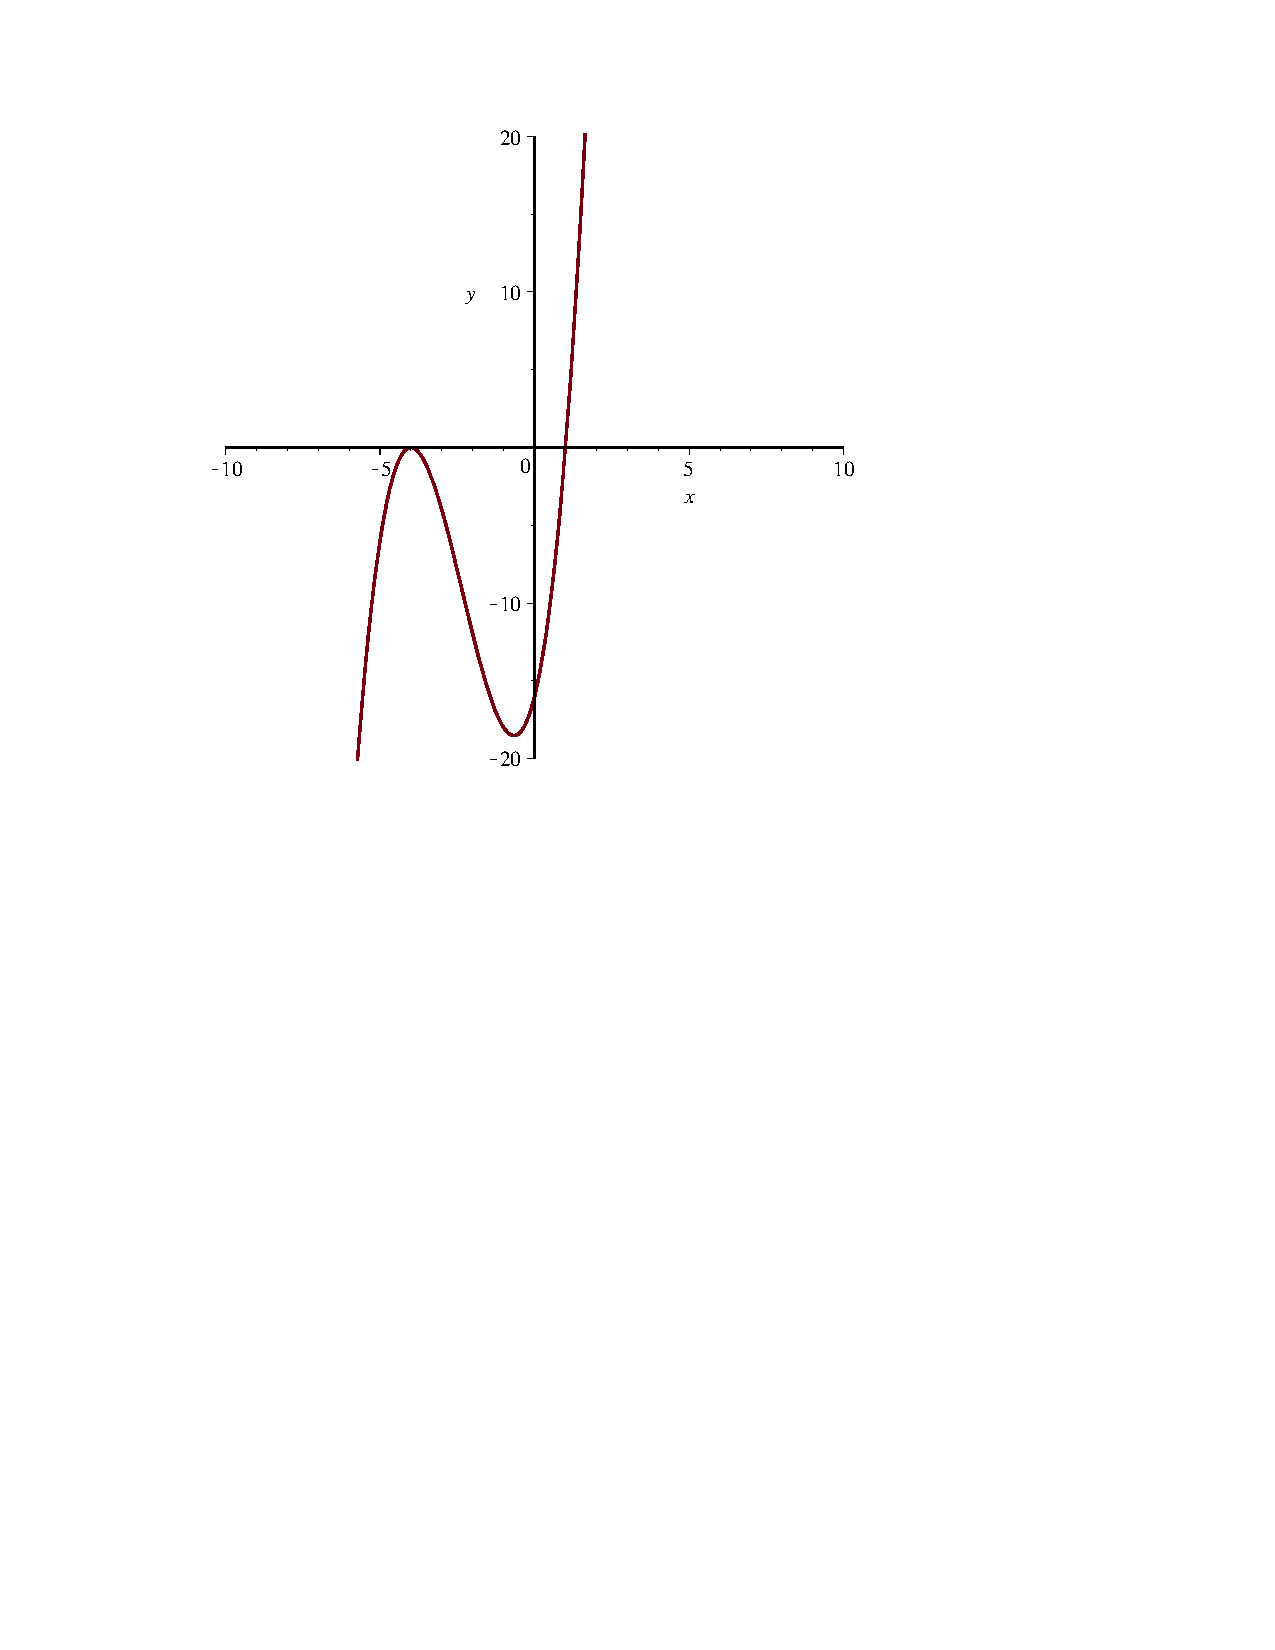
\includegraphics[scale=0.25]{2.pdf}
\end{center}
}}

\item $f(x)=\frac{x}{x+2}$

\fbox{\parbox{1\linewidth}{\begin{center}
$f(x)=\frac{x}{x+2}$; $f^{\prime}(x)=\frac{2}{(x+2)^2}$; $f^{\prime \prime}(x)=-\frac{4}{(x+2)^3}$\\
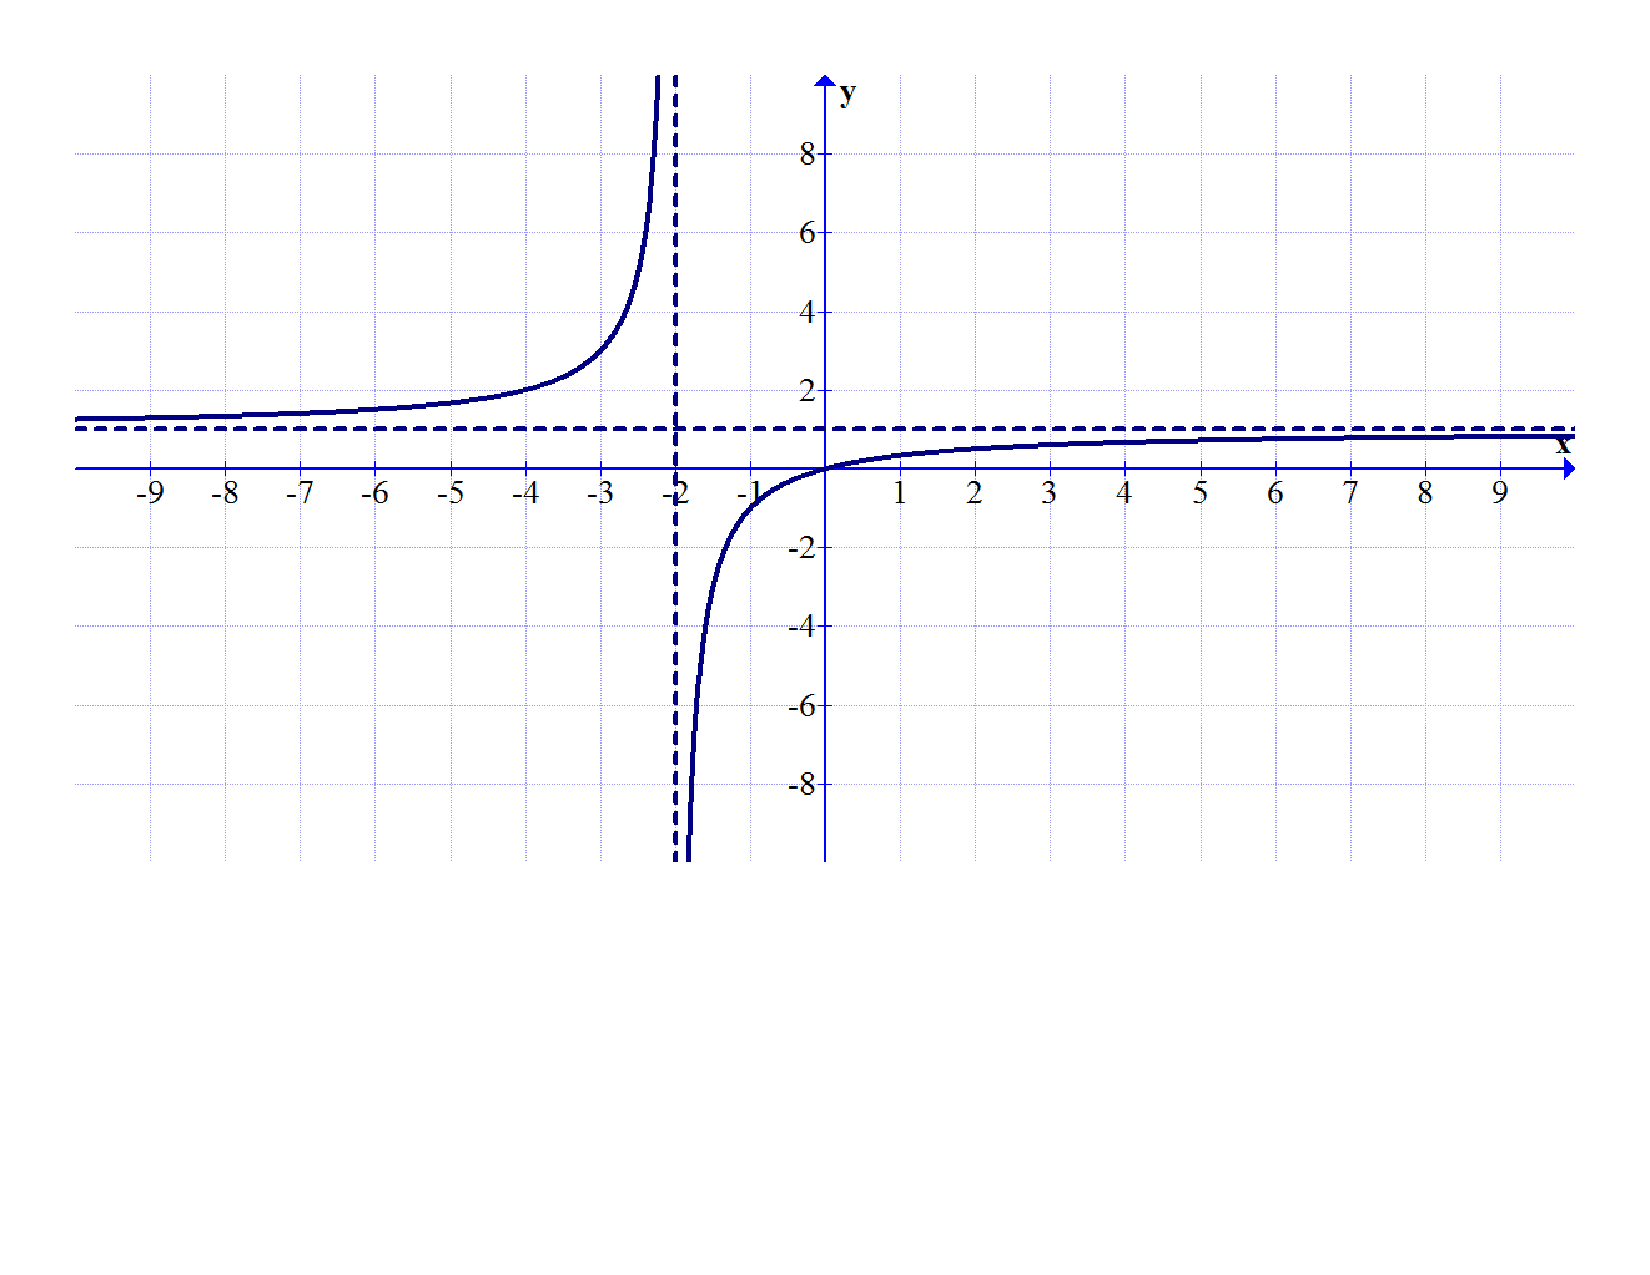
\includegraphics[scale=0.25]{3.pdf}
\end{center}
}}

\item $f(x)=\frac{x^2+x}{x^2-1}$

\fbox{\parbox{1\linewidth}{\begin{center}
$f(x)=\frac{x^2+x}{x^2-1}$; $f^{\prime}(x)=-\frac{1}{(x-1)^2}$; $f^{\prime \prime}(x)=\frac{2}{(x-1)^3}$\\
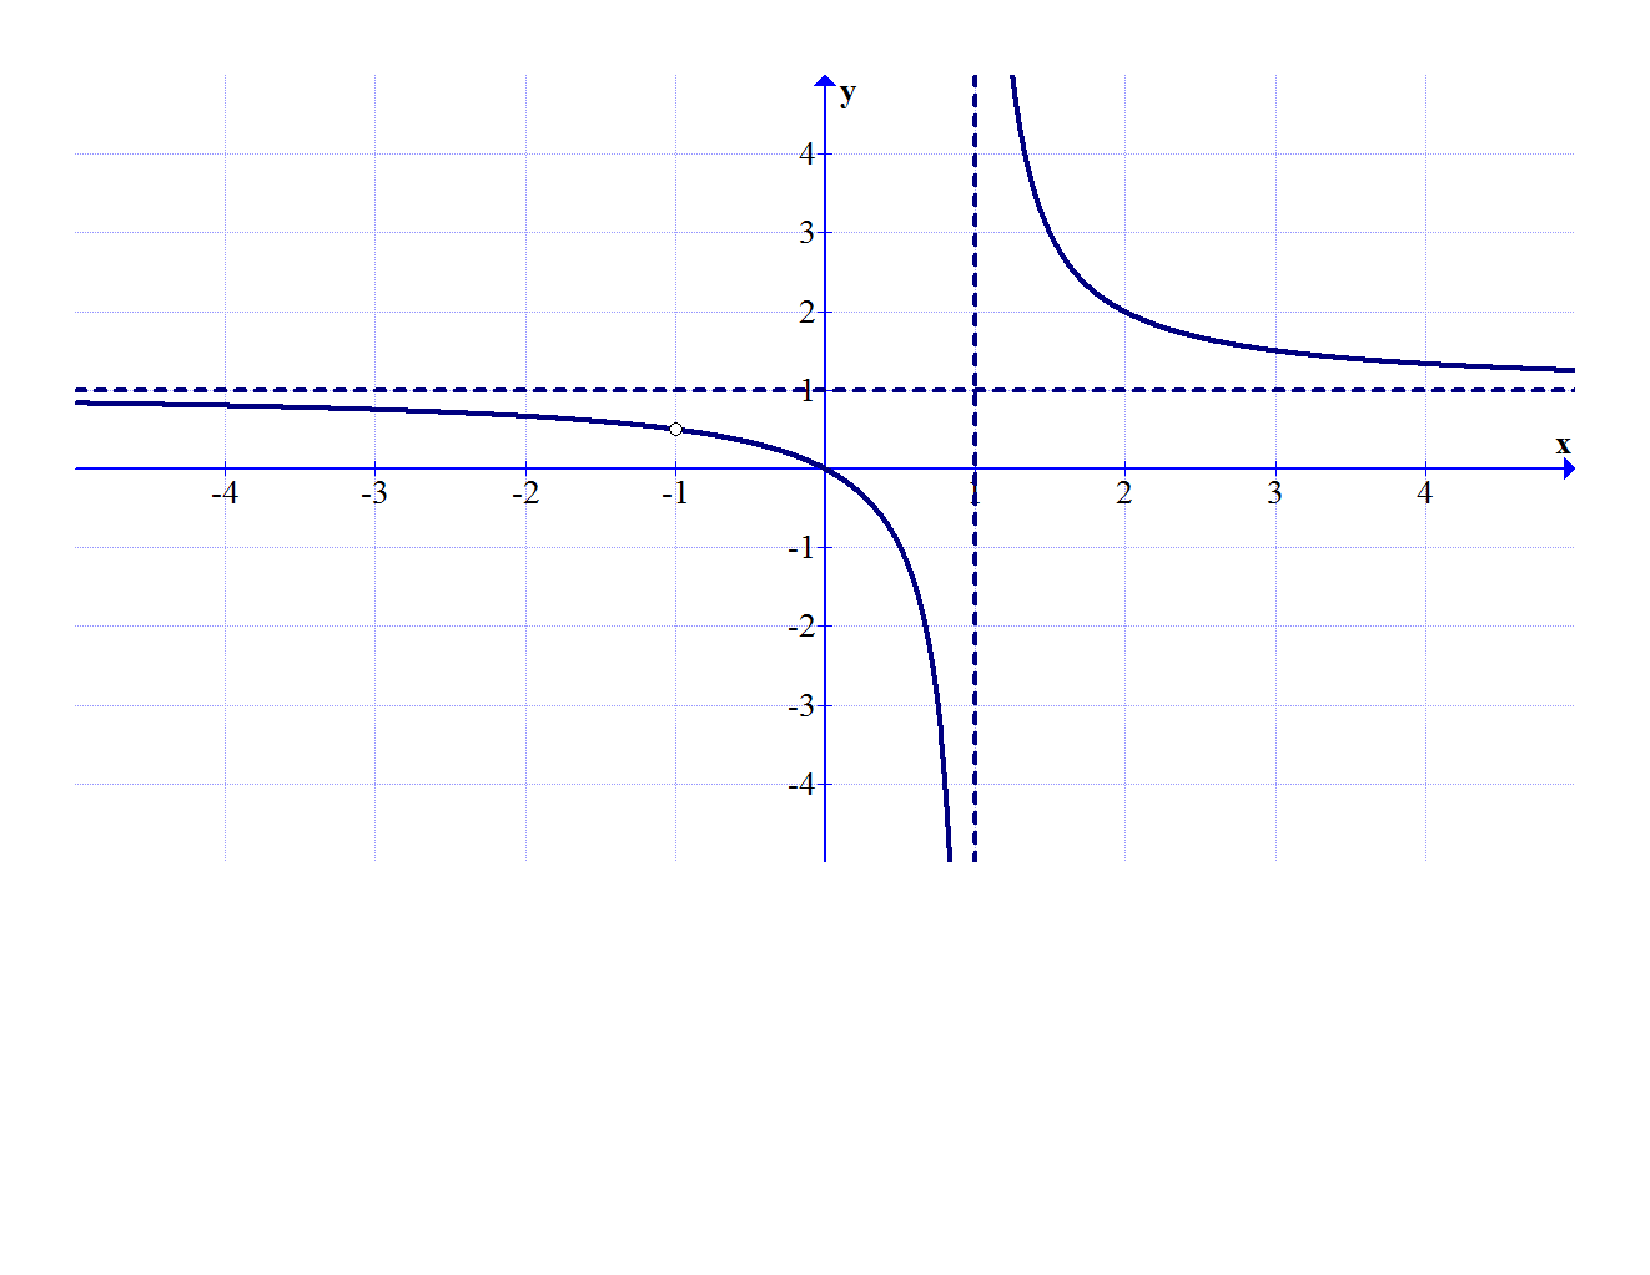
\includegraphics[scale=0.25]{4.pdf}\\
NOTE: There is a hole in the graph at the point $\left(-1,\frac{1}{2}\right)$
\end{center}
}}

\item $f(x)=\frac{x}{x^2+2}$

\fbox{\parbox{1\linewidth}{\begin{center}
$f(x)=\frac{x}{x^2+2}$; $f^{\prime}(x)=\frac{2-x^2}{(x^2+2)^2}$; $f^{\prime \prime}(x)=\frac{2x(x^2-6)}{(x^2+2)^3}$\\
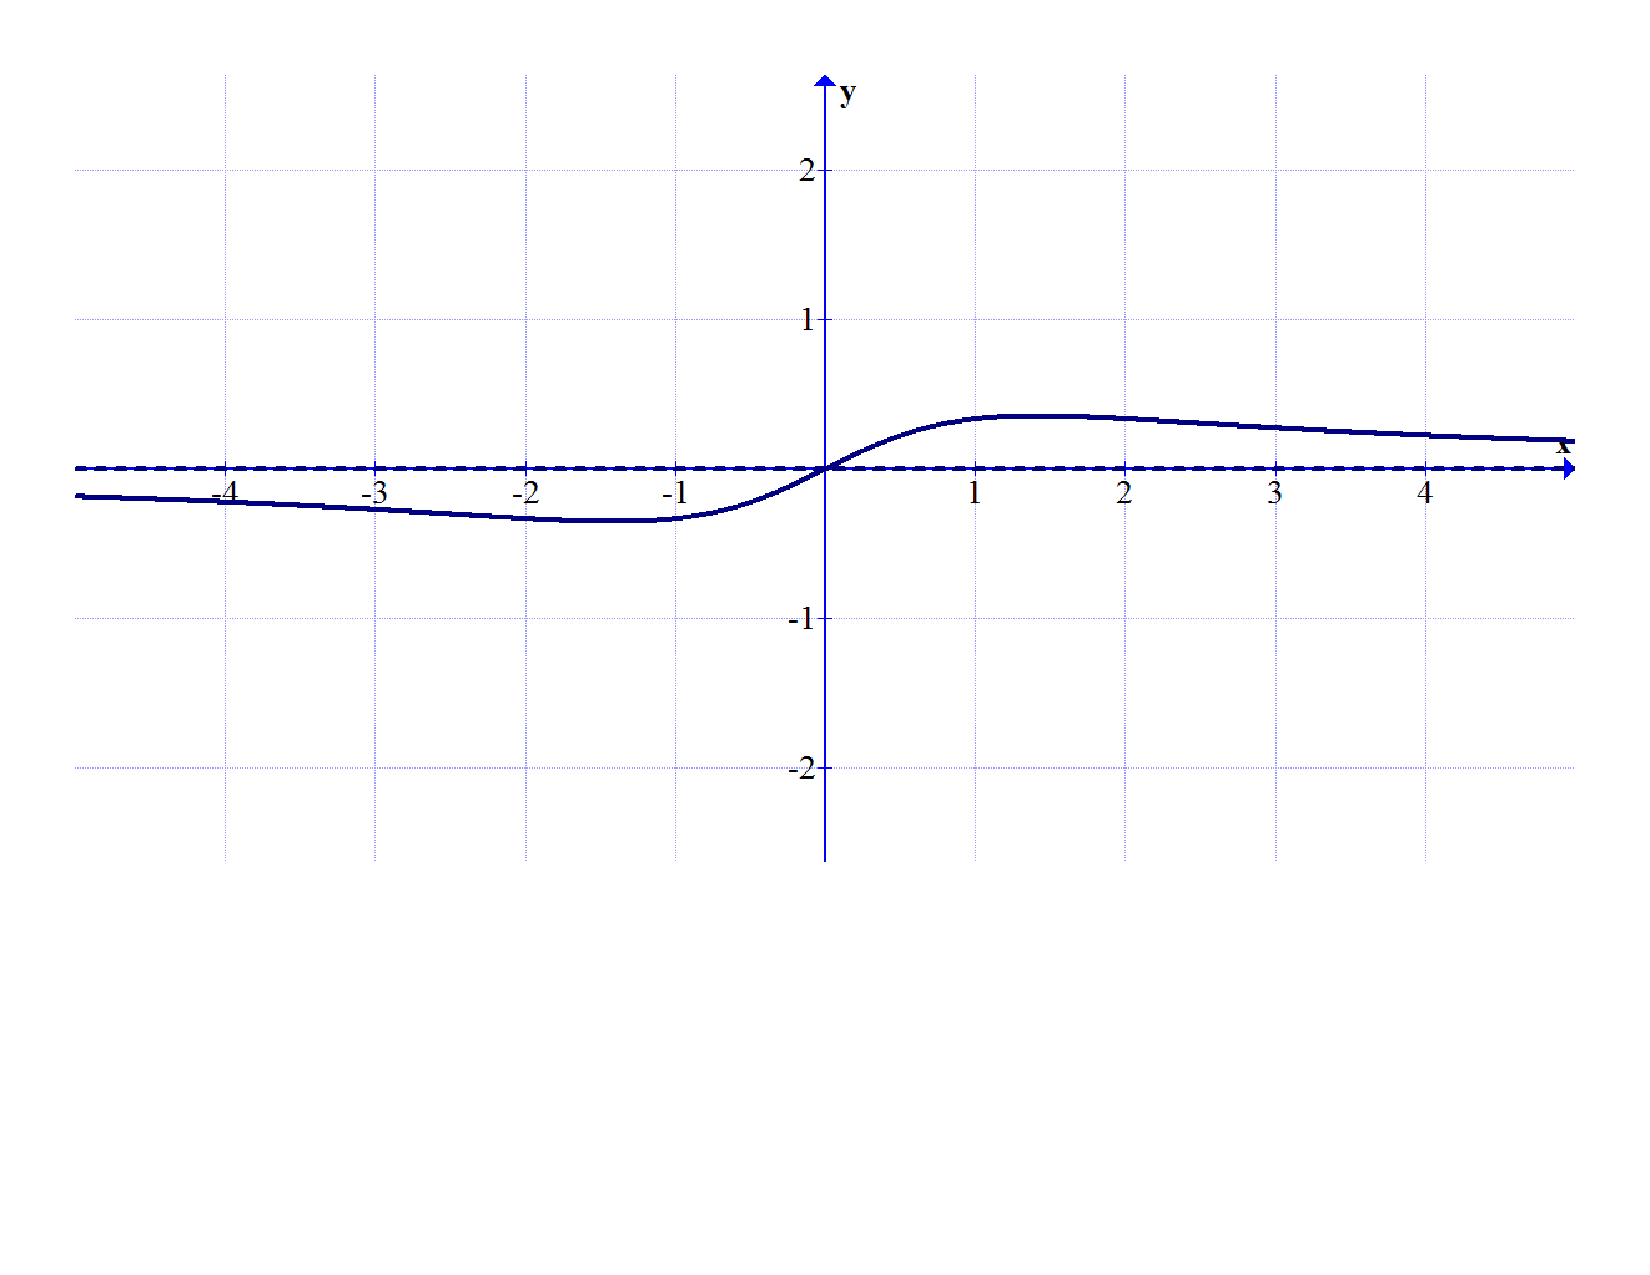
\includegraphics[scale=0.25]{5.pdf}
\end{center}
}}

\newpage

\item $f(x)=\frac{x}{x^2-4}$

\fbox{\parbox{1\linewidth}{\begin{center}
$f(x)=\frac{x}{x^2-4}$; $f^{\prime}(x)=-\frac{x^2+4}{(x^2-4)^2}$; $f^{\prime \prime}(x)=\frac{2x(x^2+12)}{(x^2-4)^3}$\\
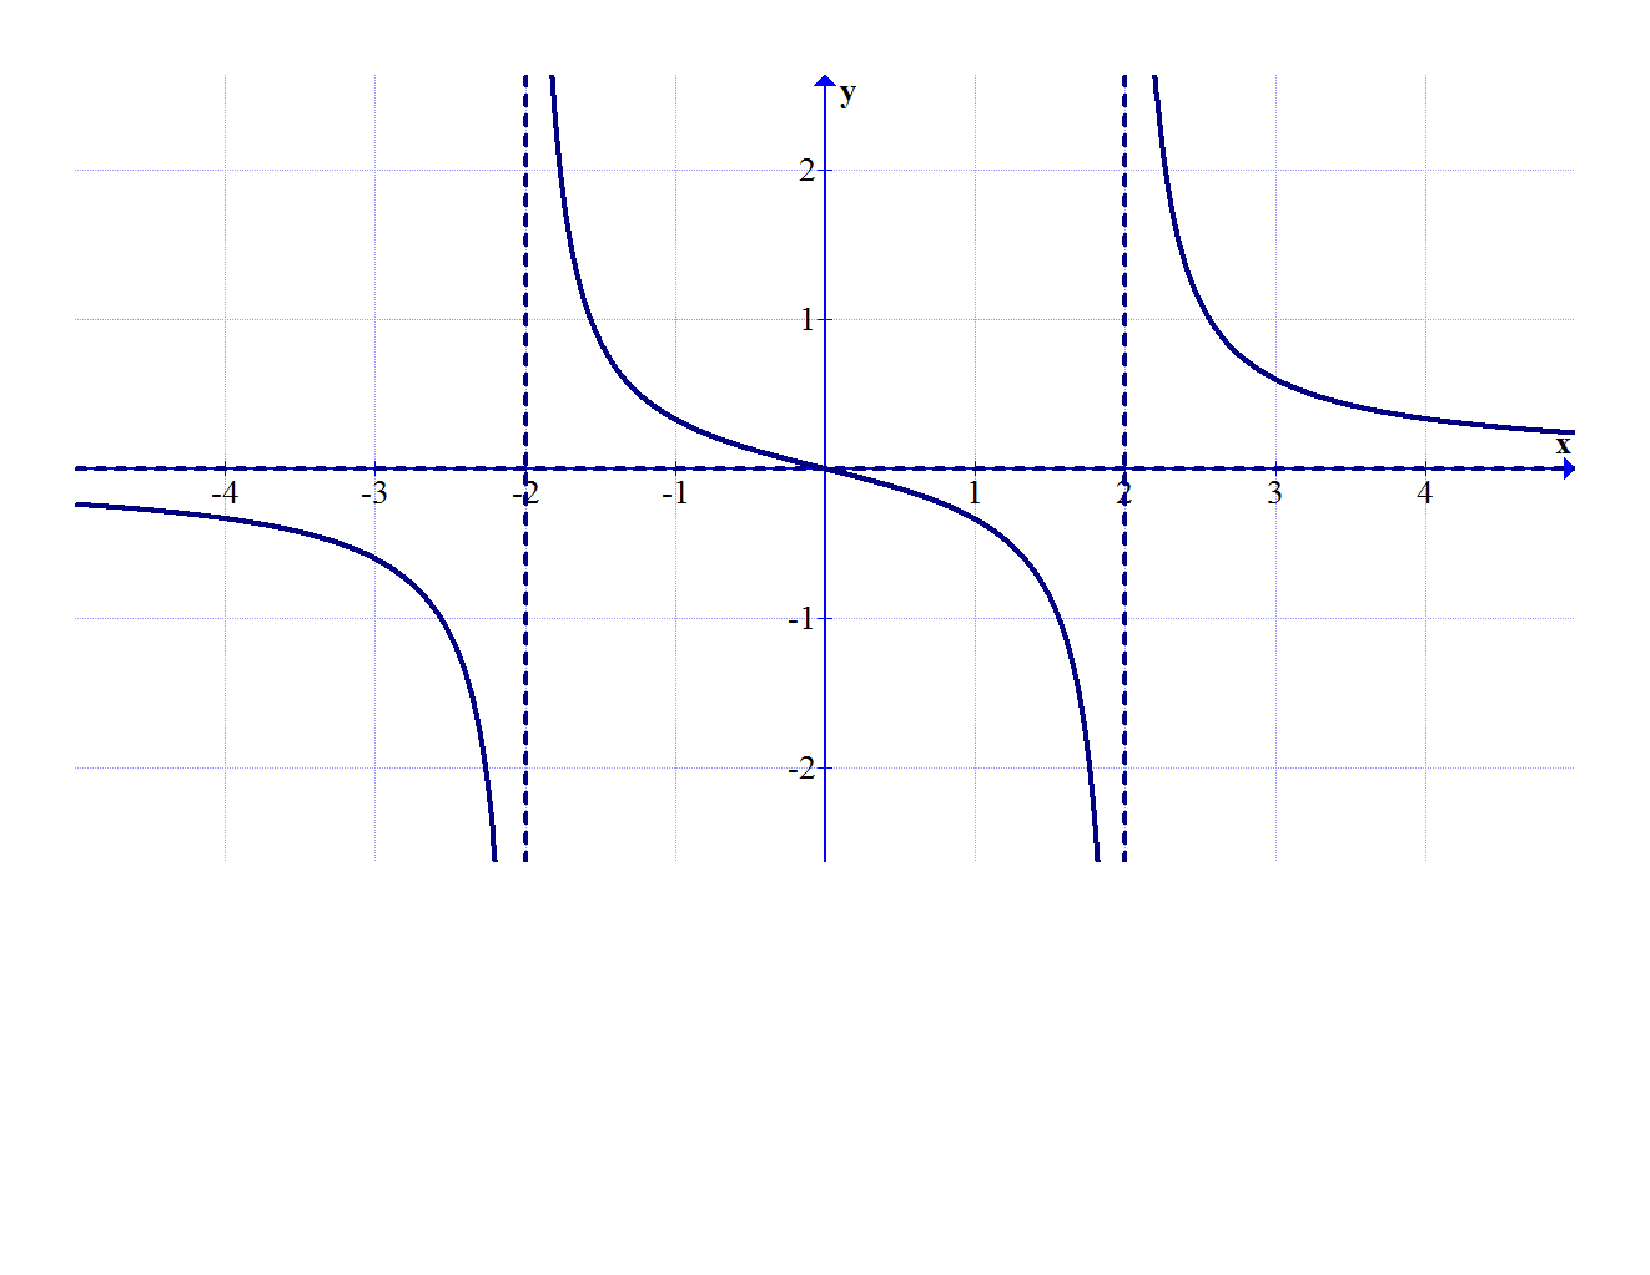
\includegraphics[scale=0.25]{6.pdf}
\end{center}
}}

\item $f(x)=xe^{2x}$

\fbox{\parbox{1\linewidth}{\begin{center}
$f(x)=xe^{2x}$; $f^{\prime}(x)=e^{2x}(2x+1)$; $f^{\prime \prime}(x)=4e^{2x}(x+1)$\\
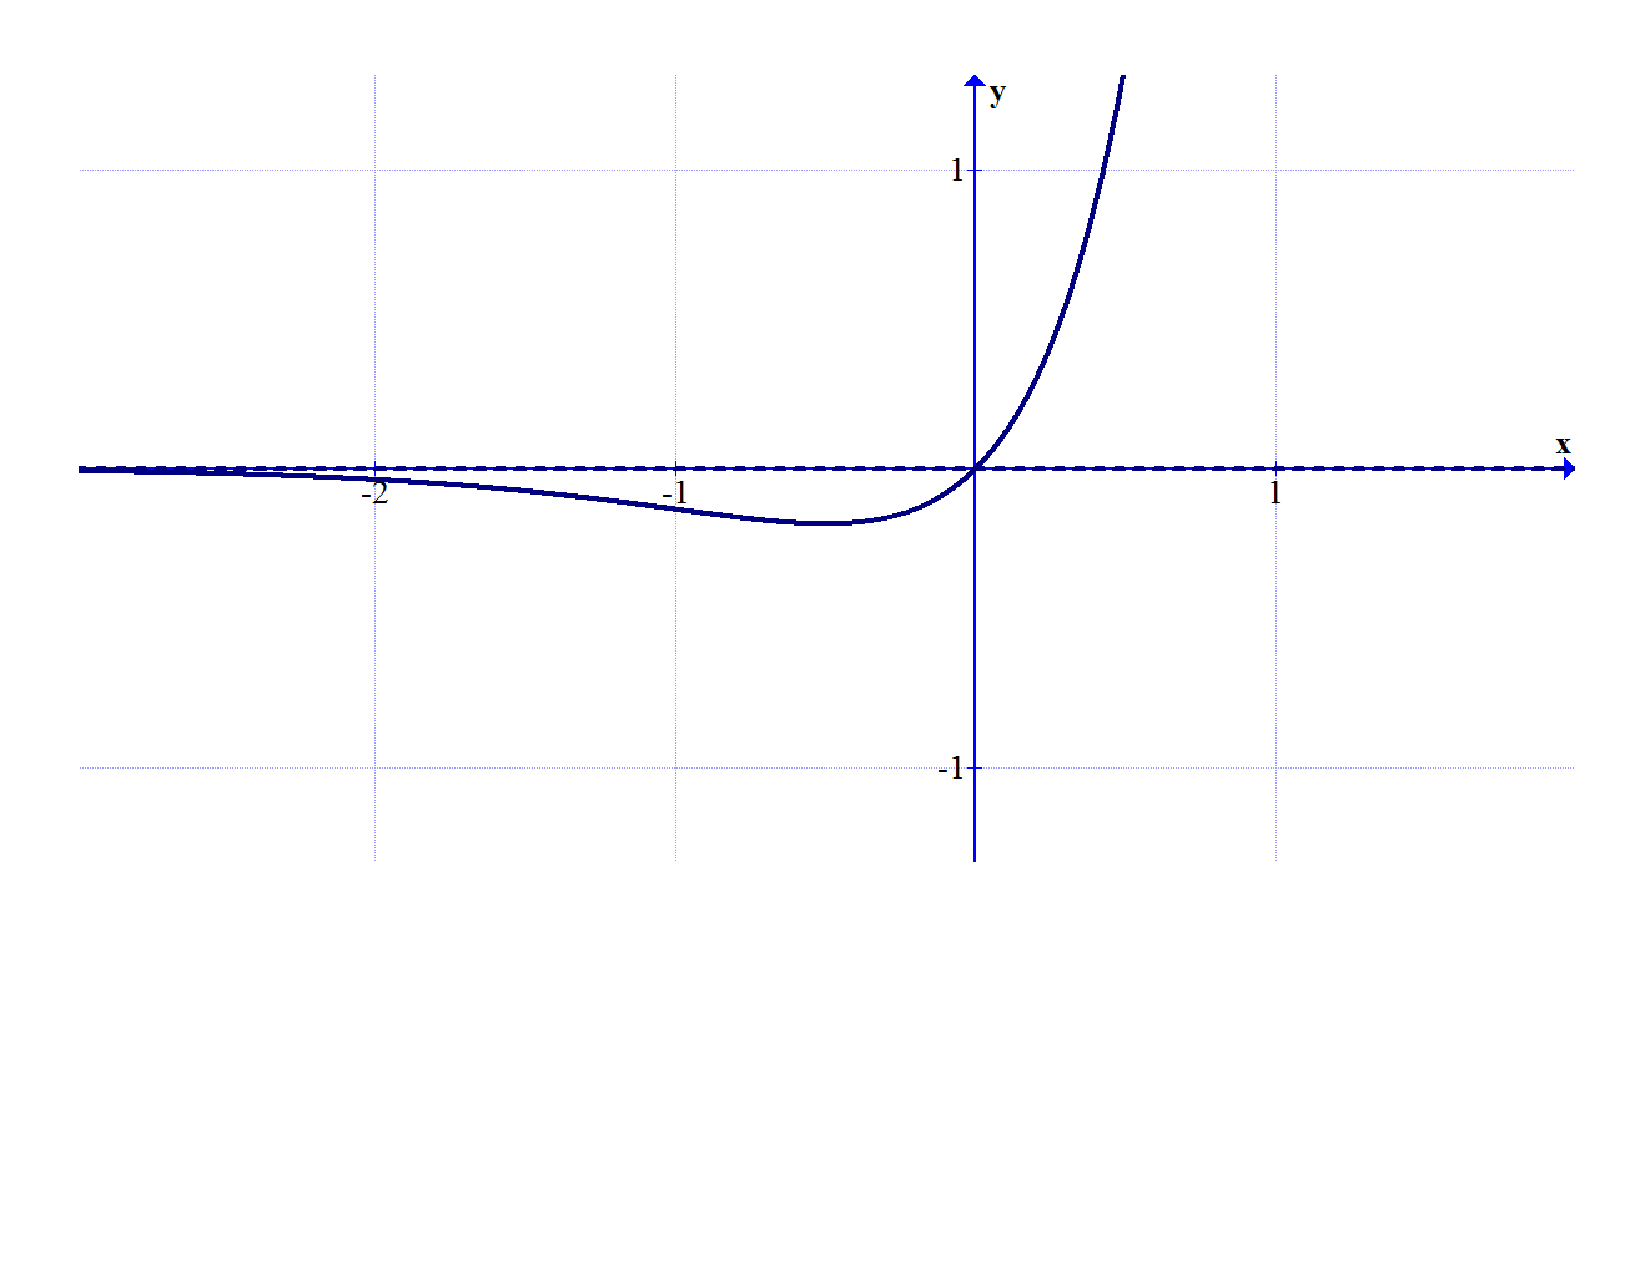
\includegraphics[scale=0.25]{7.pdf}
\end{center}
}}

\item $f(x)=\frac{1}{\sqrt{2\pi}}e^{-x^2/2}$

\fbox{\parbox{1\linewidth}{\begin{center}
$f(x)=\frac{1}{\sqrt{2\pi}}e^{-x^2/2}$; $f^{\prime}(x)=-\frac{x}{\sqrt{2\pi}}e^{-x^2/2}$; $f^{\prime \prime}(x)=\frac{1}{\sqrt{2\pi}}e^{-x^2/2}(x^2-1)$\\
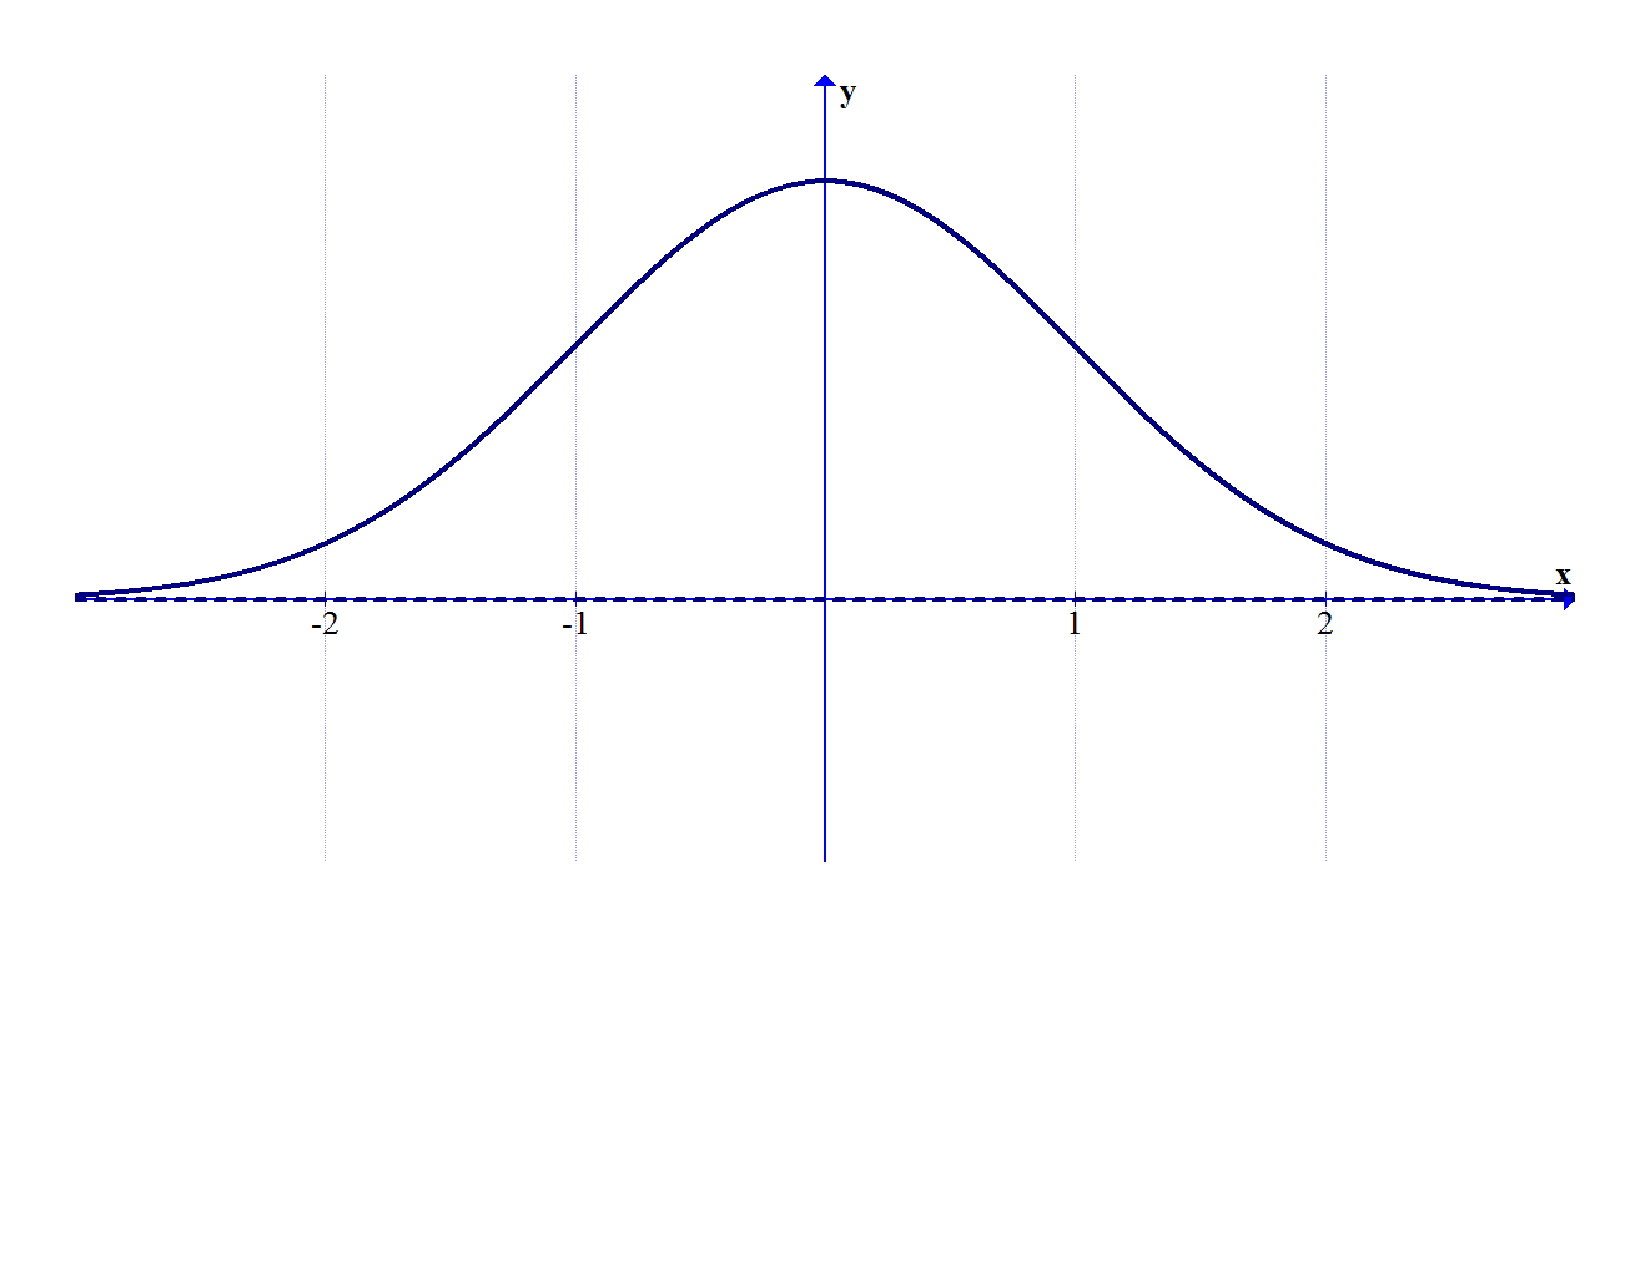
\includegraphics[scale=0.25]{8.pdf}
\end{center}
}}

\newpage

\item $f(x)=\frac{\ln{x}}{x}$

\fbox{\parbox{1\linewidth}{\begin{center}
$f(x)=\frac{\ln{x}}{x}$; $f^{\prime}(x)=\frac{1-\ln{x}}{x^2}$; $f^{\prime \prime}(x)=\frac{-3+2\ln{x}}{x^3}$\\
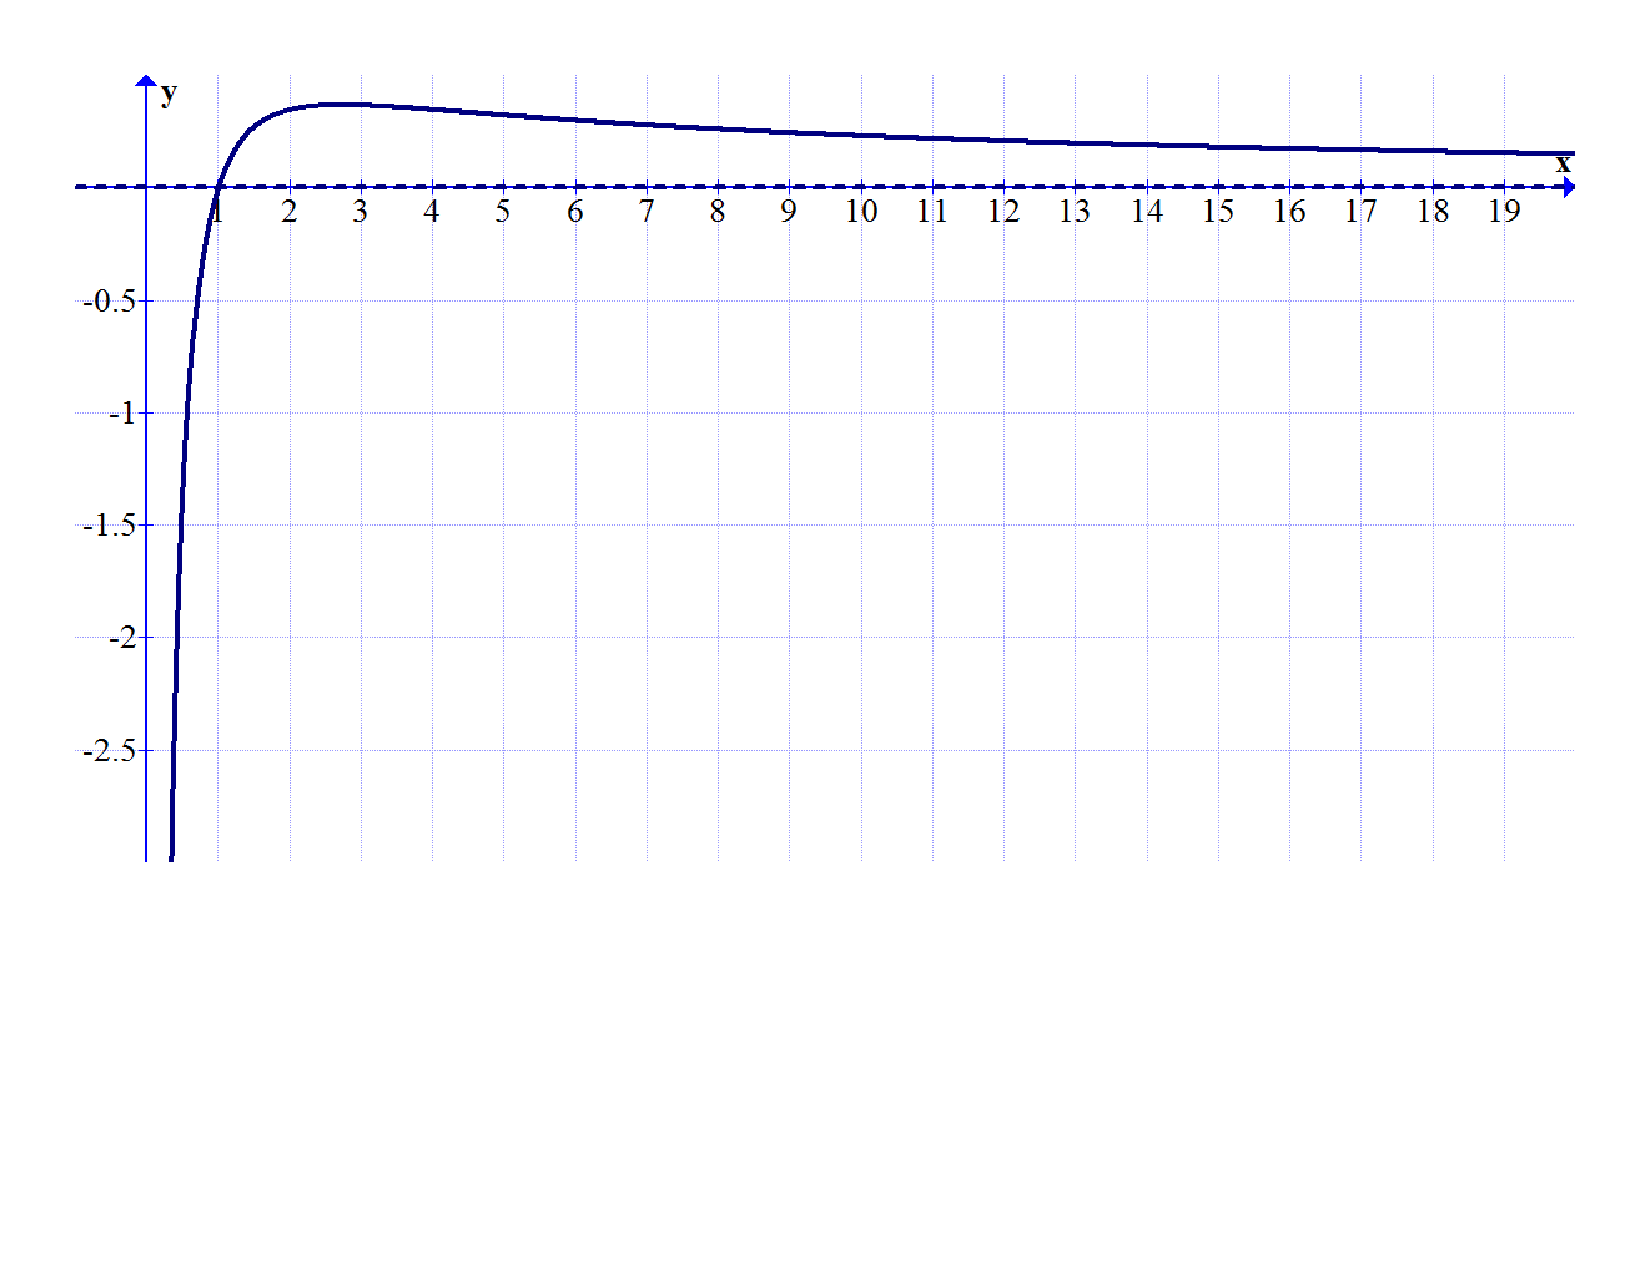
\includegraphics[scale=0.25]{9.pdf}
\end{center}
}}

\item $f(x)=x^{2/3}(x+15)$

\fbox{\parbox{1\linewidth}{\begin{center}
$f(x)=x^{2/3}(x+15)$; $f^{\prime}(x)=\frac{5(x+6)}{3x^{1/3}}$; $f^{\prime \prime}(x)=\frac{10(x-3)}{9x^{4/3}}$\\
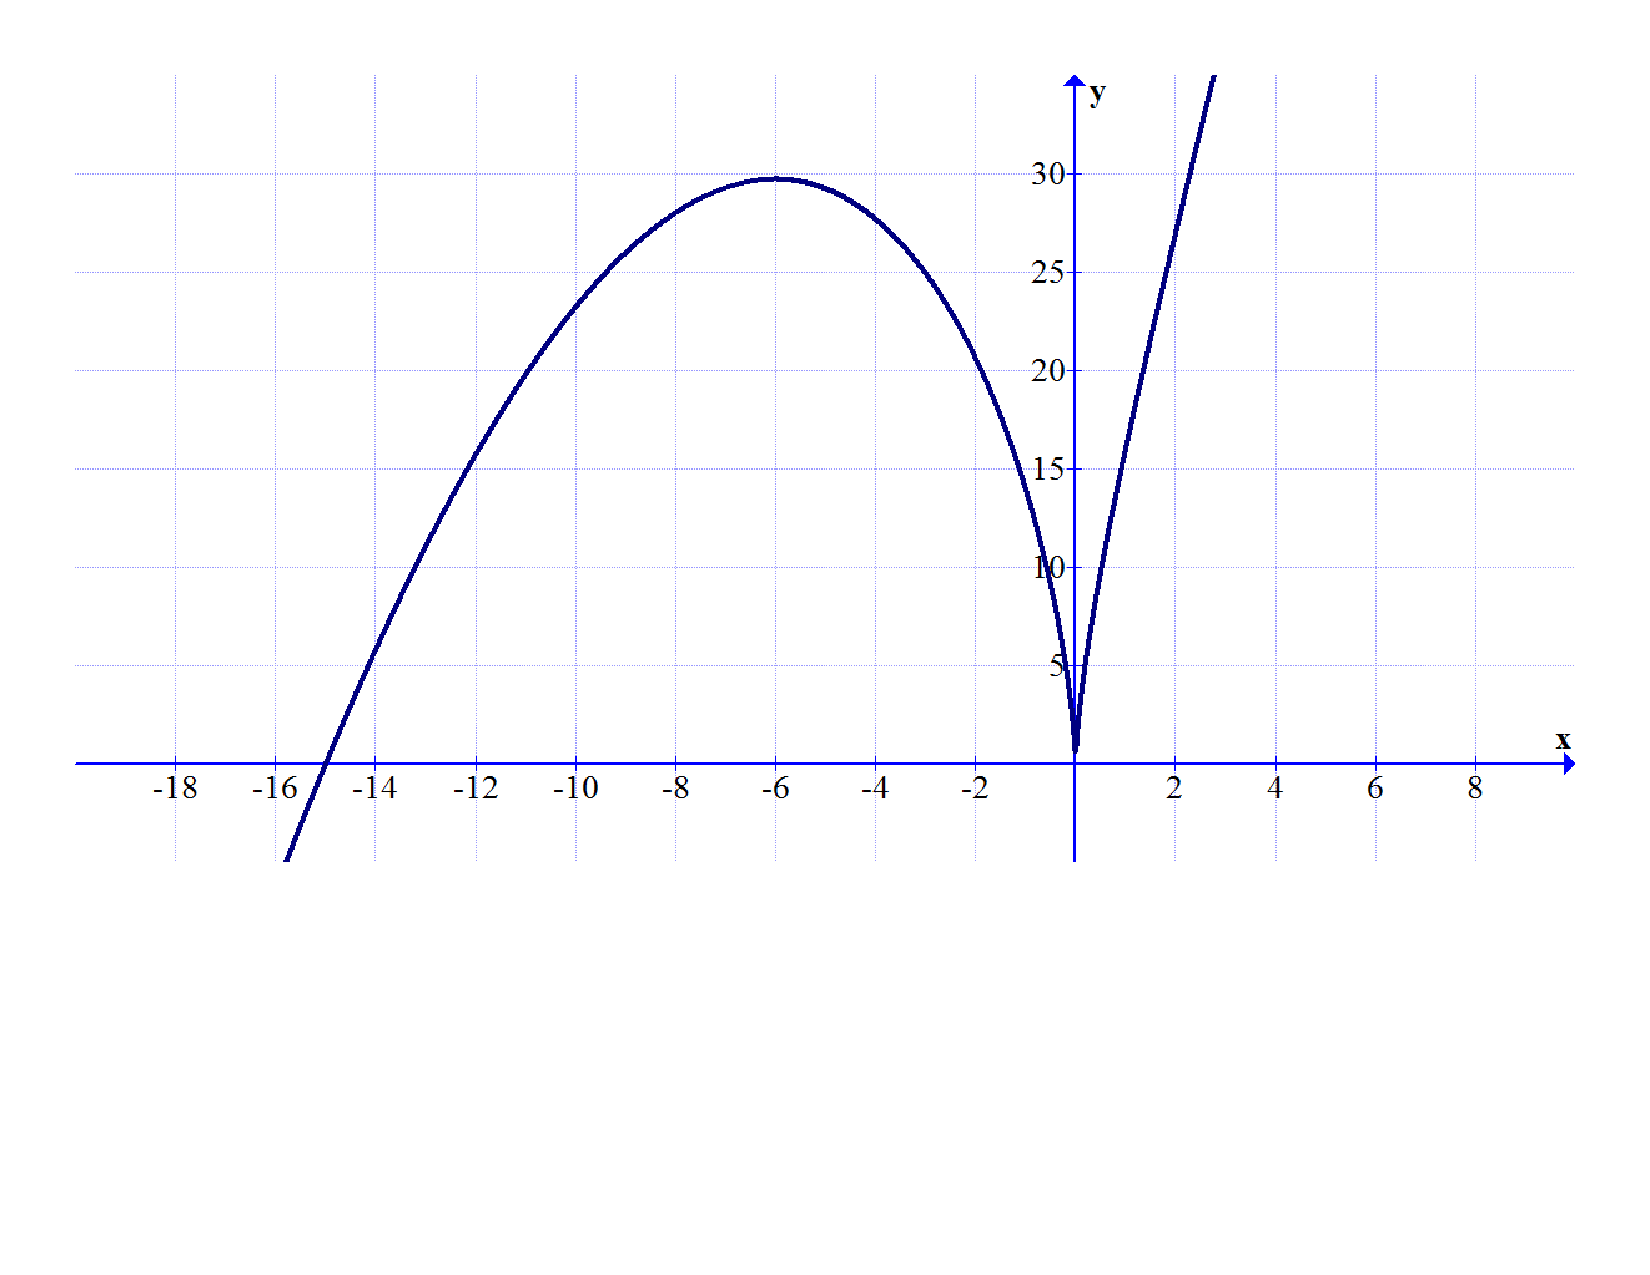
\includegraphics[scale=0.25]{10.pdf}
\end{center}
}}

\item $f(x)=4x-\tan{x}$ on $\left[-\frac{\pi}{2},\frac{\pi}{2}\right]$

\fbox{\parbox{1\linewidth}{\begin{center}
$f(x)=4x-\tan{x}$; $f^{\prime}(x)=4-\sec^2{x}$; $f^{\prime \prime}(x)=-2\sec^2{(x)}\tan{(x)}$\\
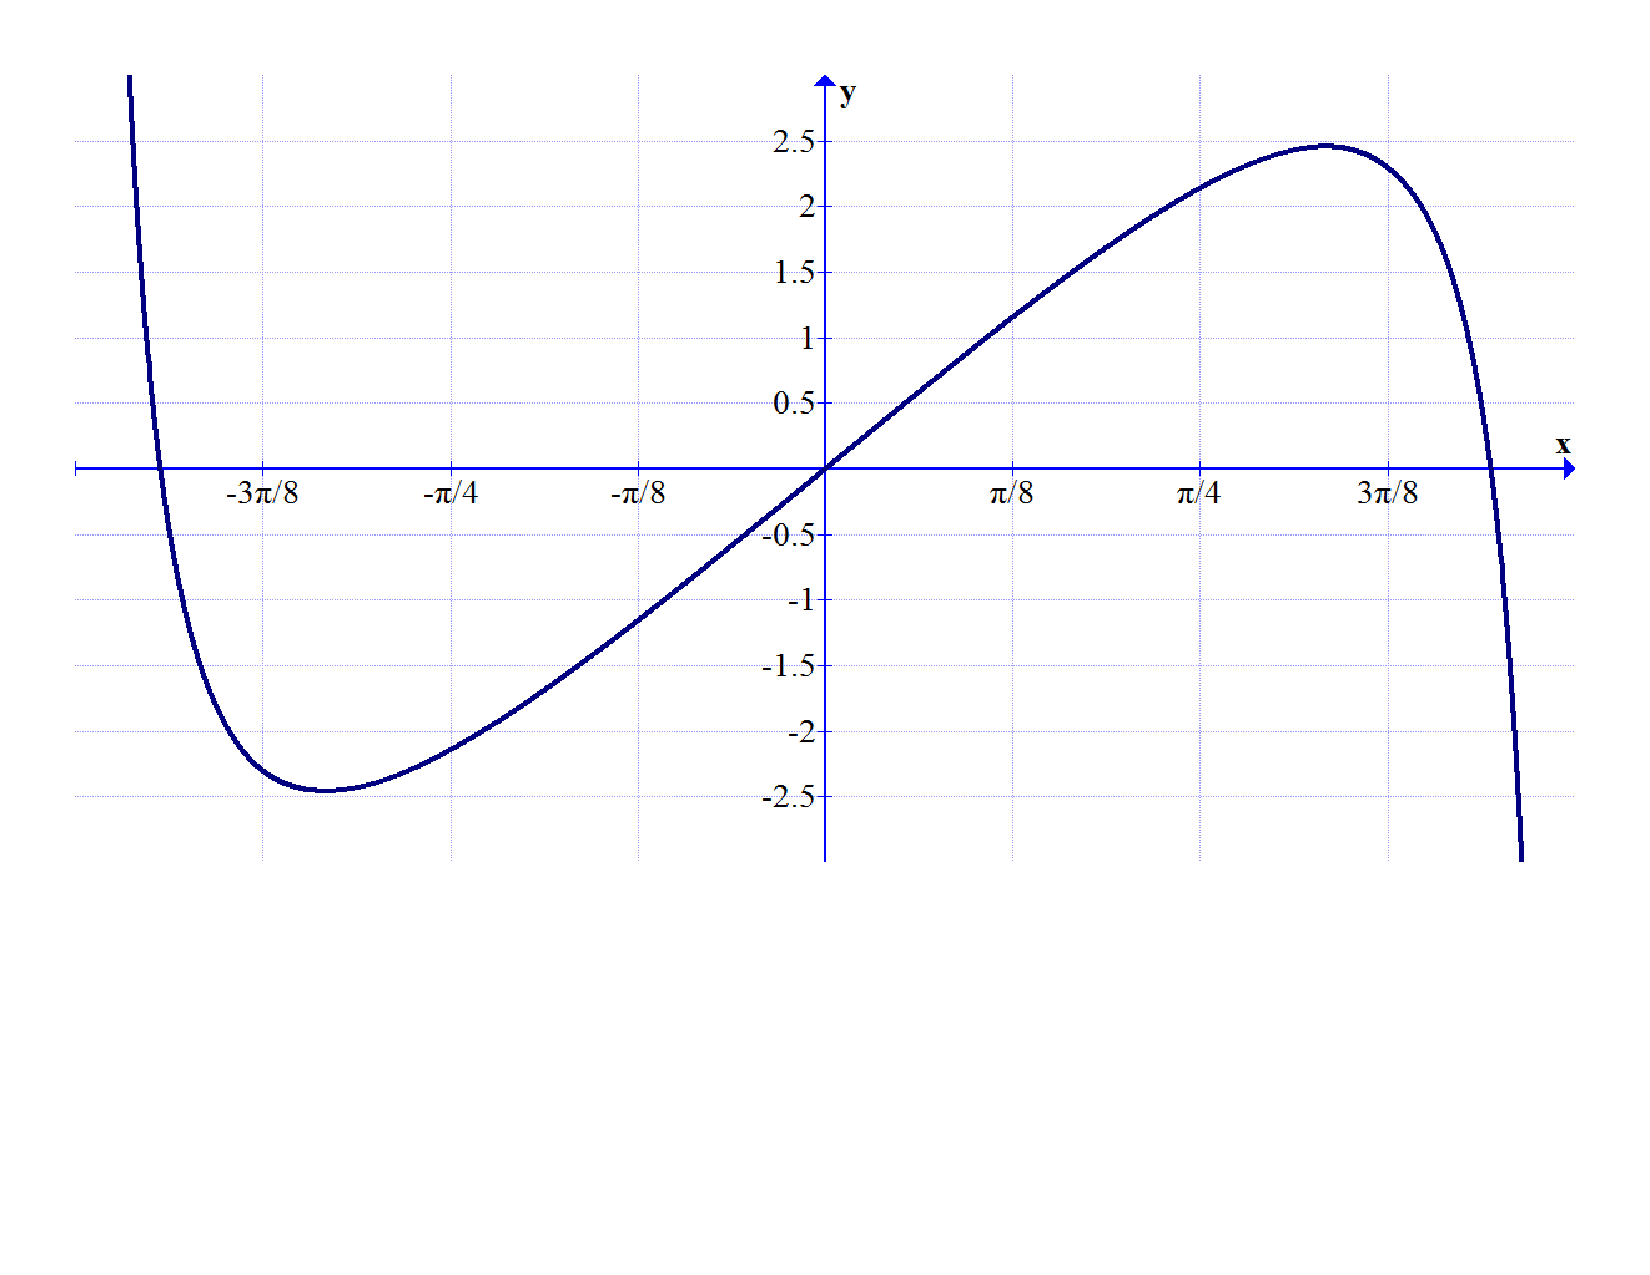
\includegraphics[scale=0.25]{11.pdf}
\end{center}
}}

\newpage

\item $f(x)=\sin^{2}{(x)}$ on $[0,2\pi]$

\fbox{\parbox{1\linewidth}{\begin{center}
$f(x)=\sin^{2}{(x)}$; $f^{\prime}(x)=2\sin{x}\cos{x}$; $f^{\prime \prime}(x)=4\cos^2{x}-2$\\
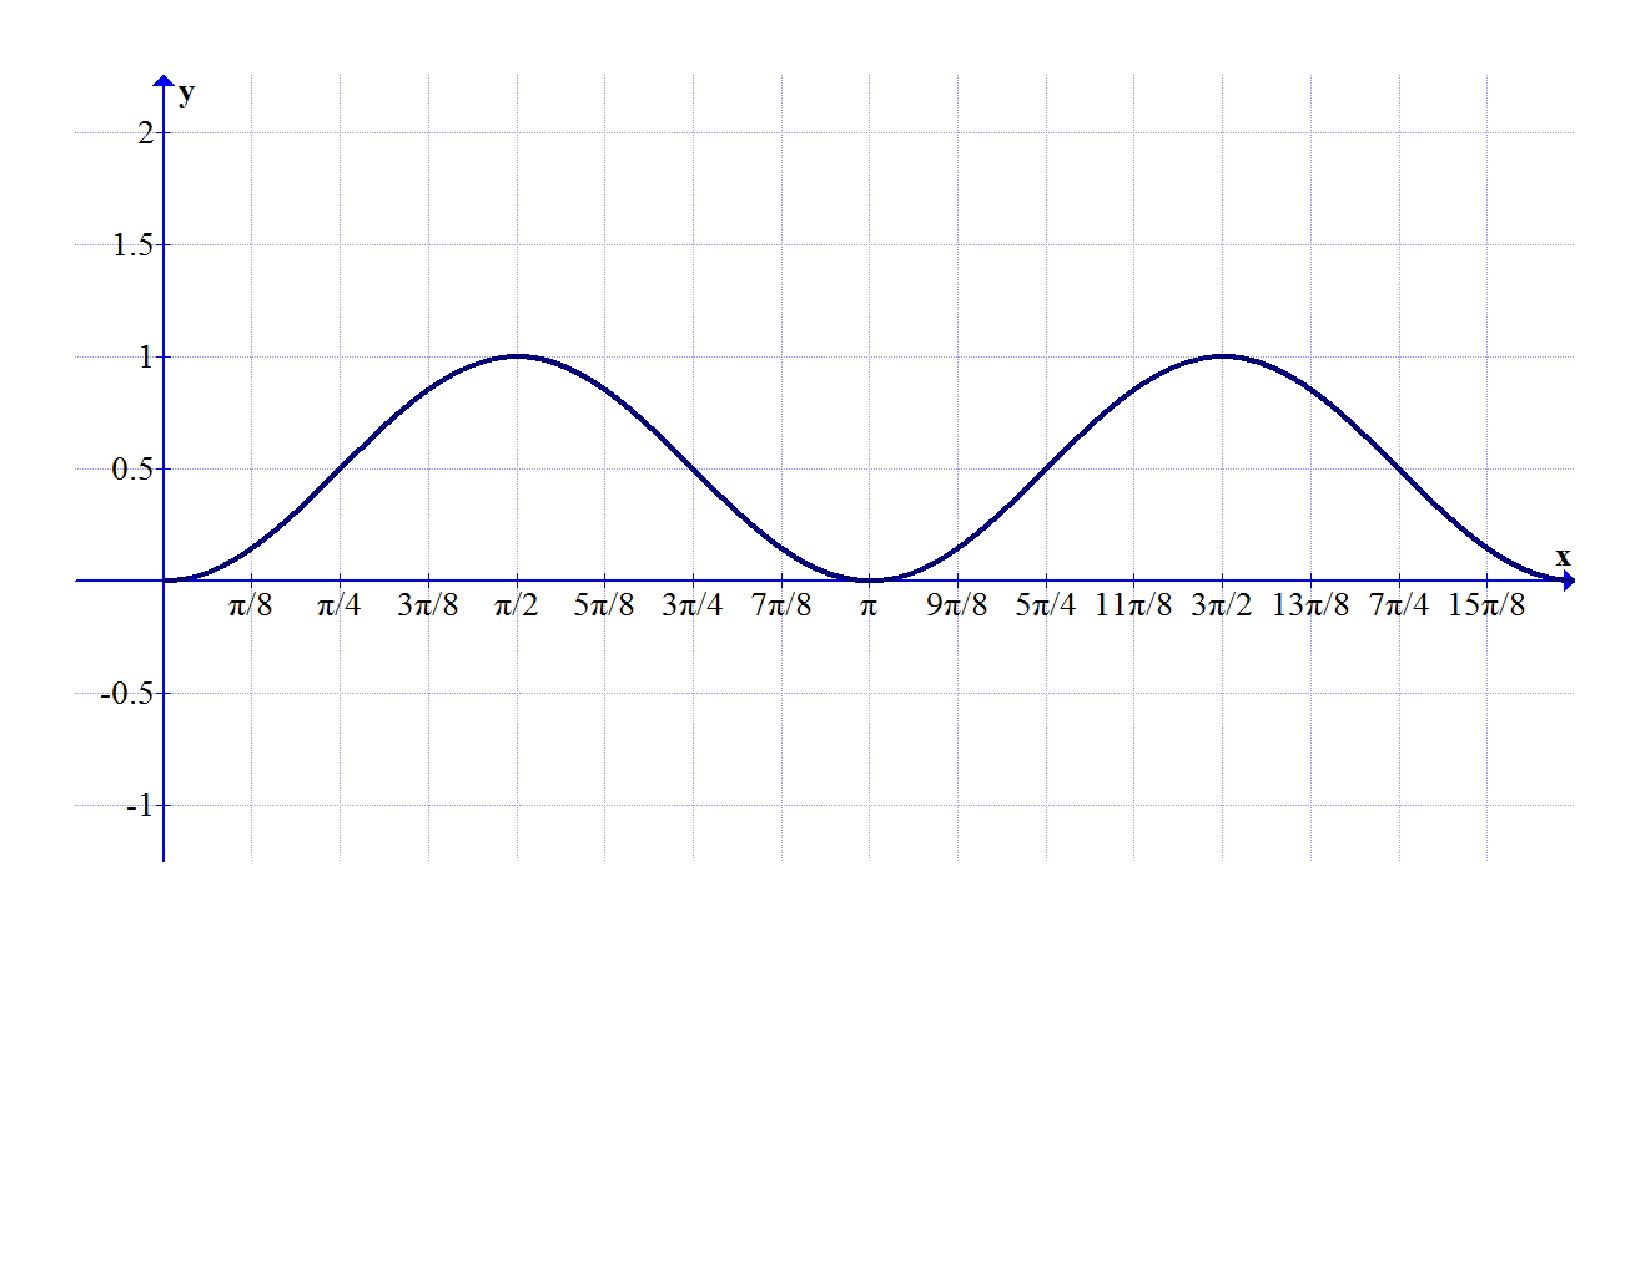
\includegraphics[scale=0.25]{12.pdf}
\end{center}
}}

\item Consider the graphs of $f(x)=x^{1/3}$ and $g(x)=x^{2/3}$.  $x_0=0$ is a critical point for both $f(x)$ and $g(x)$ since $0$ is in the domain of each function but $f^{\prime}(0)$ and $g^{\prime}(0)$ are both undefined.  How does the behavior of $f(x)$ differ from that of $g(x)$ at this critical point?

\fbox{\parbox{1\linewidth}{\begin{center}
\begin{tabular}{c|c}
$f(x)=x^{1/3}$ & $g(x)=x^{2/3}$\\ 
\hline
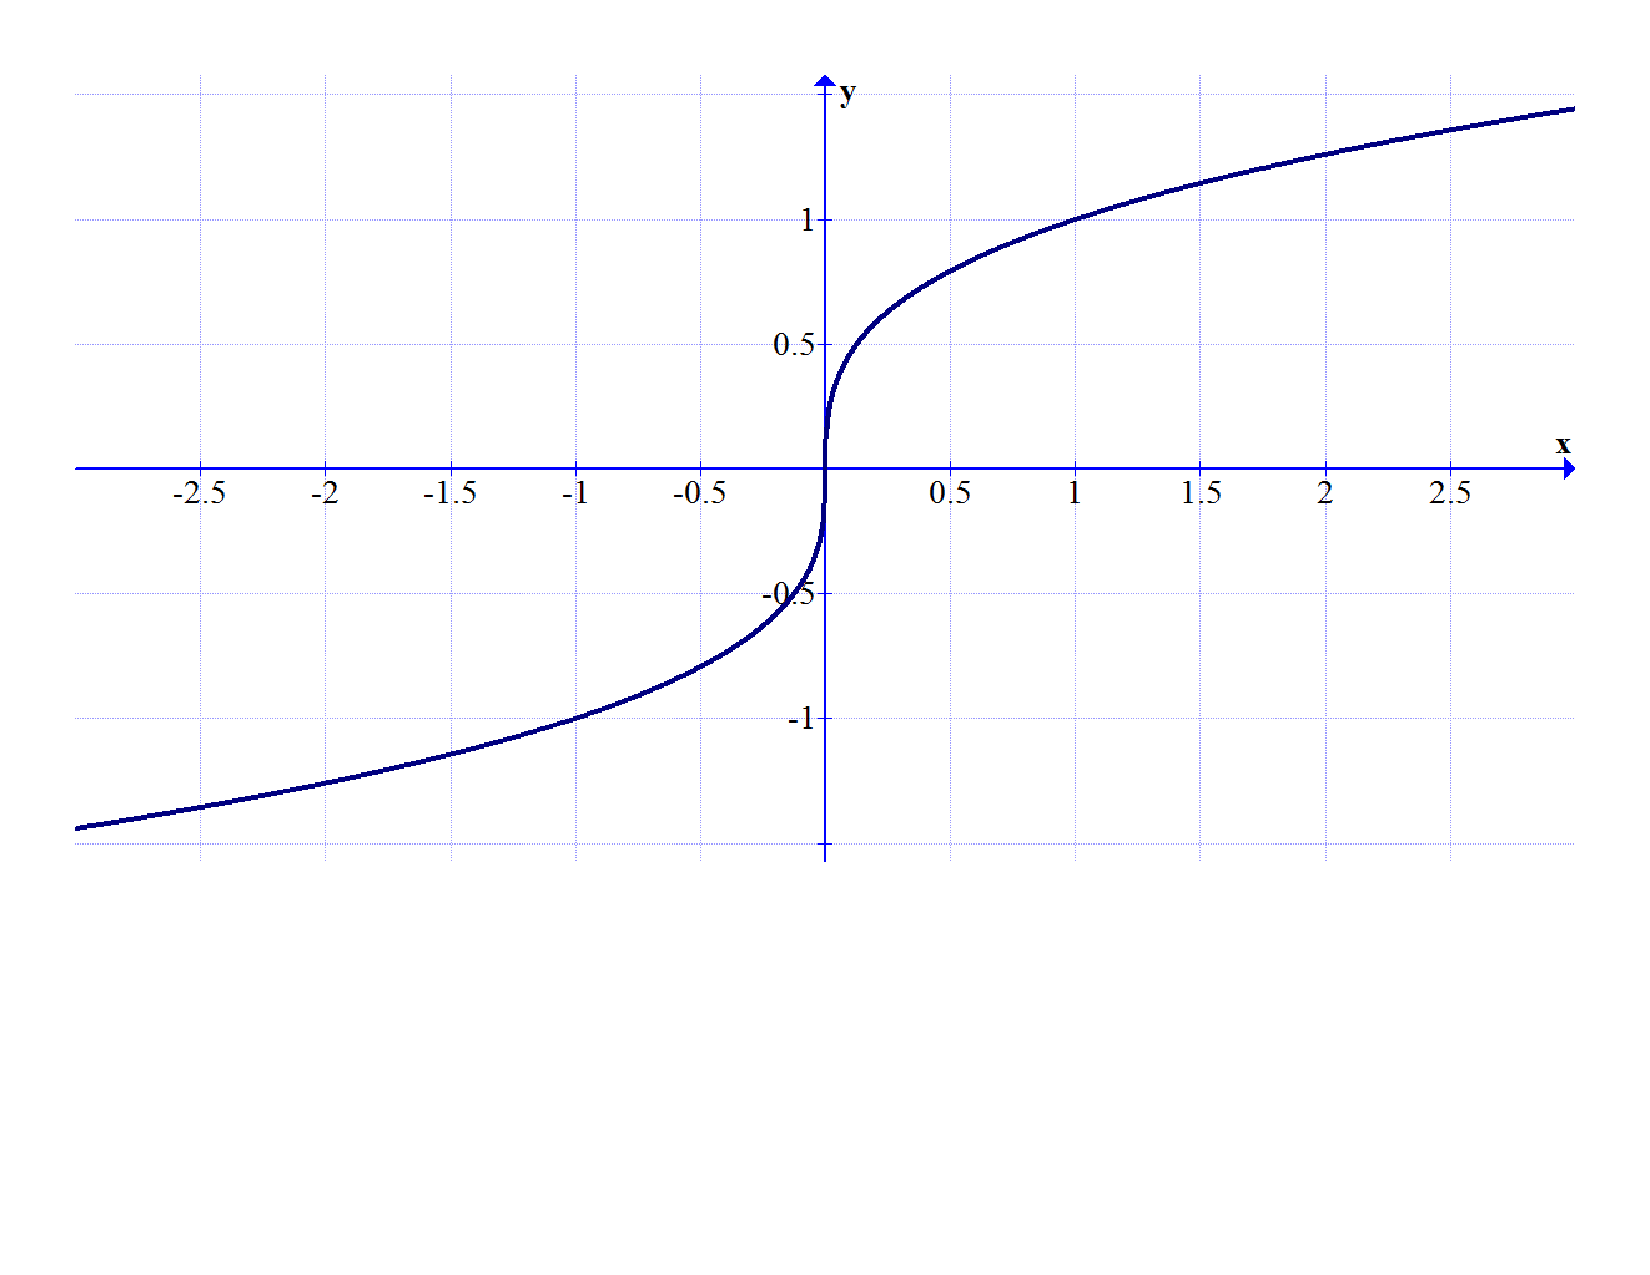
\includegraphics[scale=0.25]{13a.pdf} & 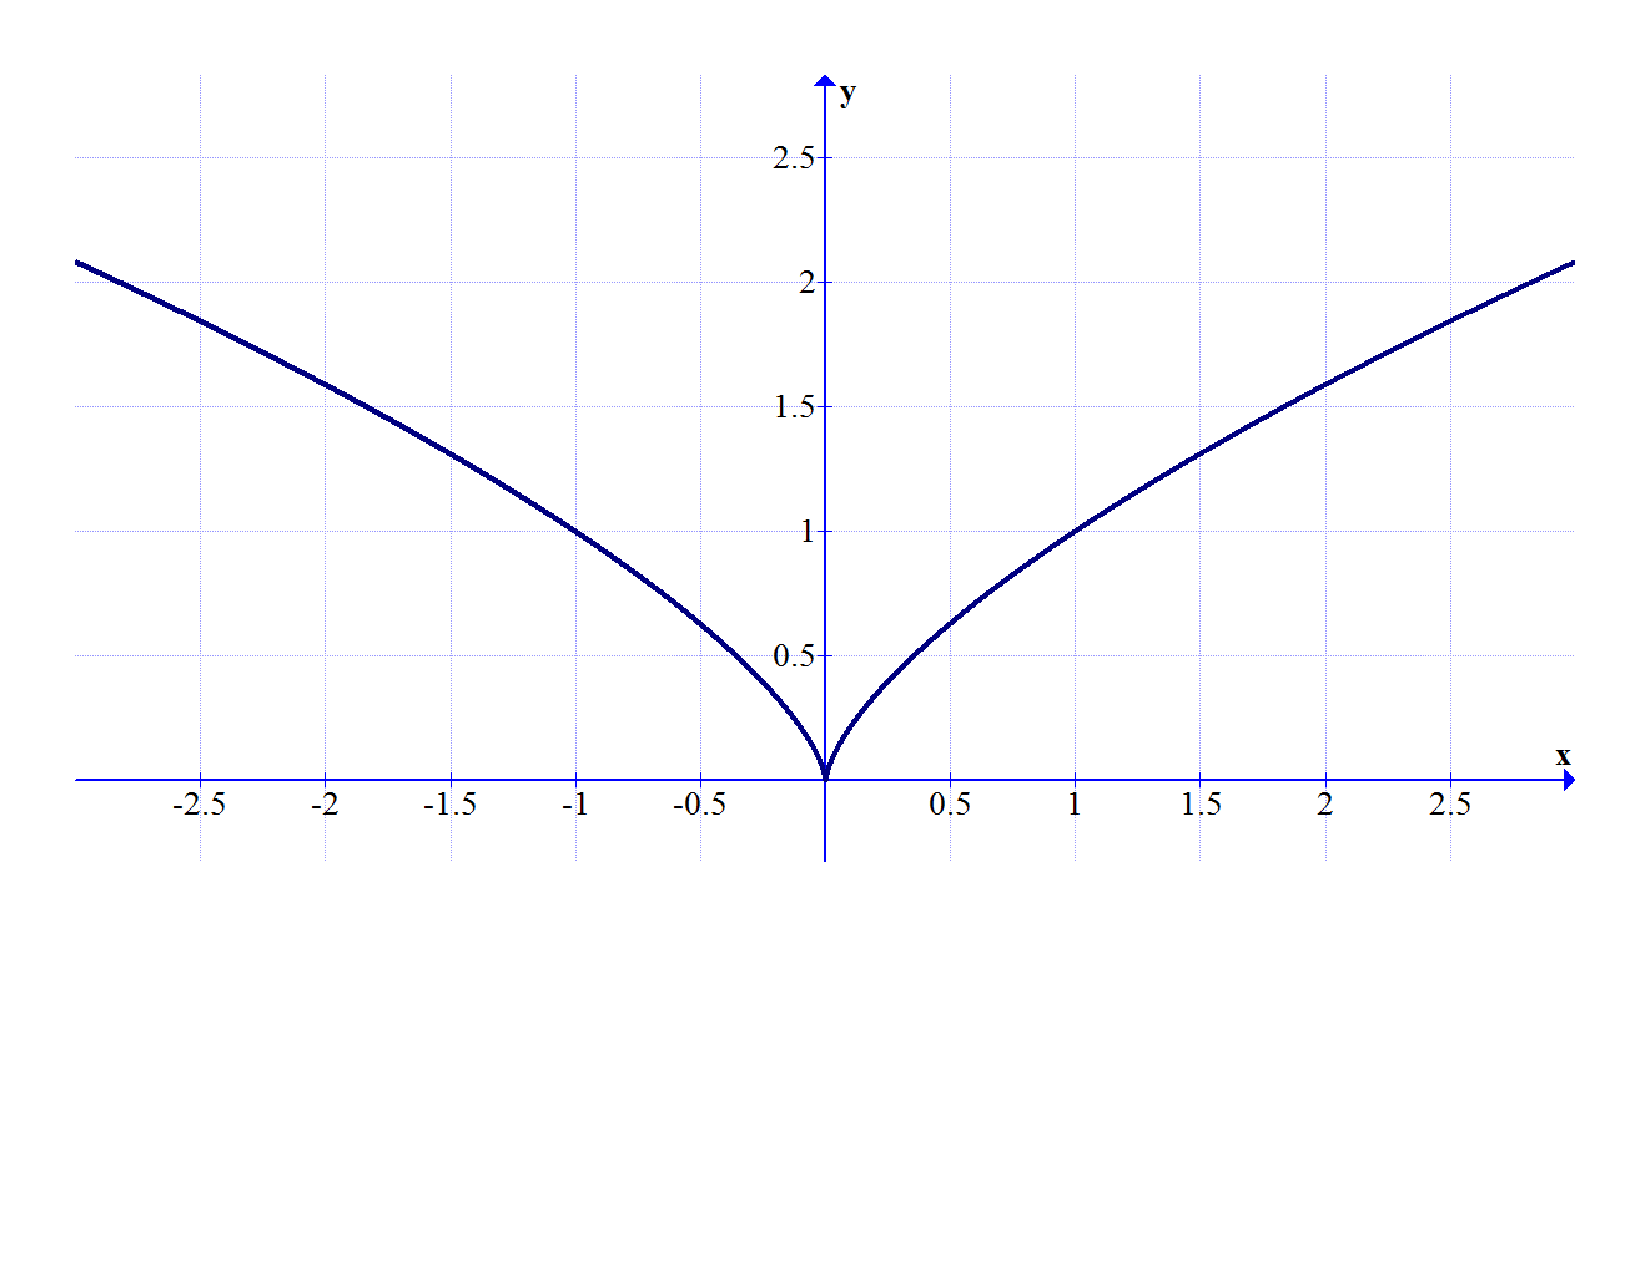
\includegraphics[scale=0.25]{13b.pdf}
\end{tabular}\\
\end{center}
In both cases, the graph has a vertical tangent line at $x=0$.  However, $g(x)$ has a cusp at $x=0$.  Also, $g(x)$ has a relative (local) minimum at this critical point, whereas $f(x)$ does not.
}}

\item Consider a general quadratic curve $f(x)=ax^2+bx+c$, where $a \neq 0$.  Show that $f(x)$ cannot have any inflection points.

\fbox{\parbox{1\linewidth}{
$f^{\prime \prime}(x)=2a$ which is always defined and never 0, since $a \neq 0$.  So, if $a>0$, $f(x)$ is always concave up; and, if $a<0$, $f(x)$ is always concave down.}}


\item Consider a general quartic curve $f(x)=ax^4+bx^3+cx^2+dx+e$, where $a \neq 0$.  

\begin{enumerate}

\item What is the largest number of distinct inflection points that $f(x)$ could have?  

\fbox{2}

\item What condition on the coefficients $a$, $b$, $c$, $d$, and $e$ is necessary for the number of distinct inflection points to be maximized?

\fbox{$a$, $b$, and $c$ must satisfy $6b^2-16ac>0$; $d$ and $e$ can be any real number.}

\end{enumerate}

\end{enumerate}

\end{document}